\section{Gleichstrom Komponenten}

\subsection{Aufbau PV-Alnage}
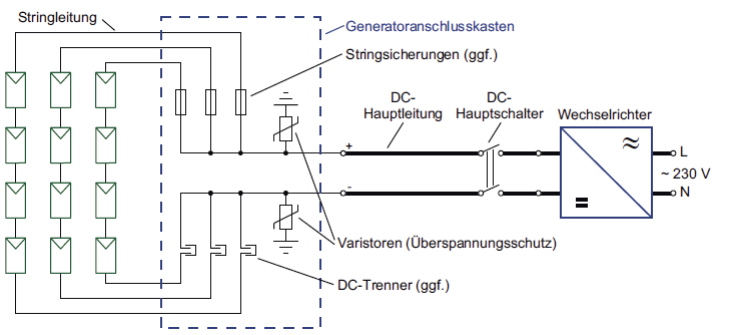
\includegraphics[width=0.95\columnwidth]{images/Aufbau_PV-Anlage.png}

\subsection{Gleichstromverkabelung}
\subsubsection{Solarstecker}

\begin{itemize}
    \item MC4 Solarstecker (quasi Standard)
\end{itemize}

\begin{minipage}[t]{0.48\columnwidth}
    \myul{\textbf{MC4}}\\
    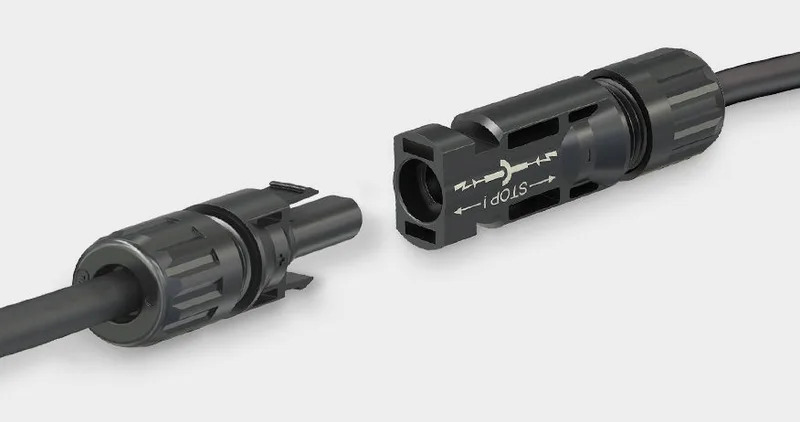
\includegraphics[width=0.95\columnwidth]{images/MC4.jpg}
\end{minipage}
\hfill
\begin{minipage}[t]{0.48\columnwidth}
    \myul{\textbf{MC4-Evo 2000}}\\
    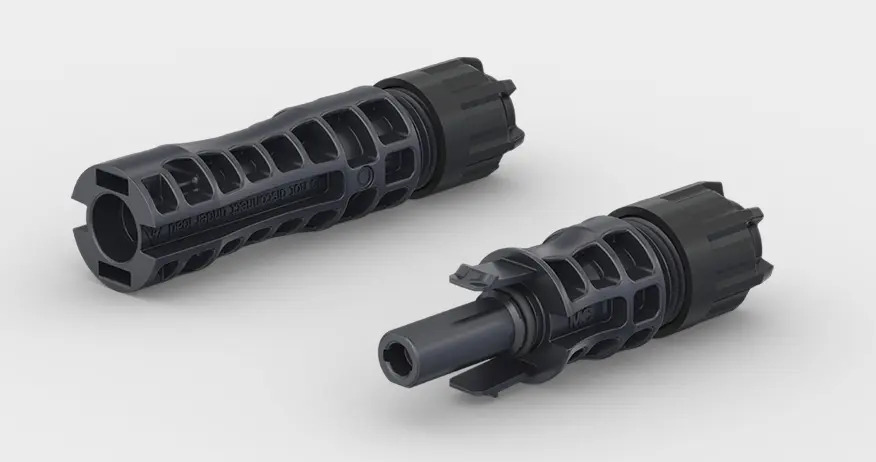
\includegraphics[width=0.95\columnwidth]{images/MC4-Evo 2000.jpg}
\end{minipage}

\vspace{0.25cm}

\subsubsection{Gleichstromkabel}

\begin{minipage}[t]{0.48\columnwidth}
    \myul{\textbf{MC FLEX-SOL-EVO-DX}}\\
    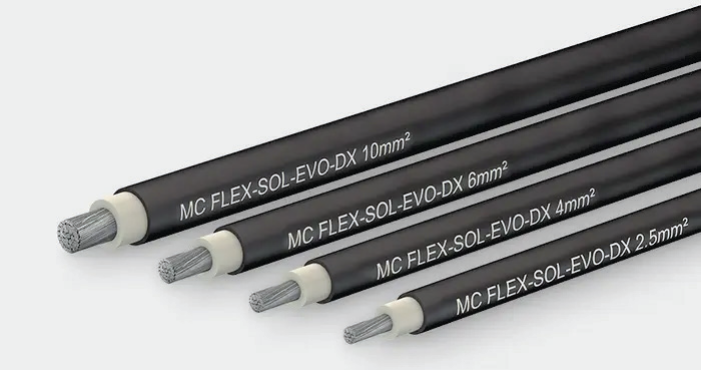
\includegraphics[width=0.95\columnwidth]{images/MC_FLEX-SOL-EVO-DX.png}
\end{minipage}
\hfill
\begin{minipage}[t]{0.48\columnwidth}
    \myul{\textbf{Anforderungen}}\\
    \begin{itemize}
        \item Doppelte Isolation\\
                (Schutz gegen Kurzschluss)
        \item UV-Beständigkeit
        \item Schwer entflammbar 
        \item Für hohe Temperaturen
\end{itemize}
\end{minipage}

\subsection{PV-Generator unter Last (fester Widerstand)}
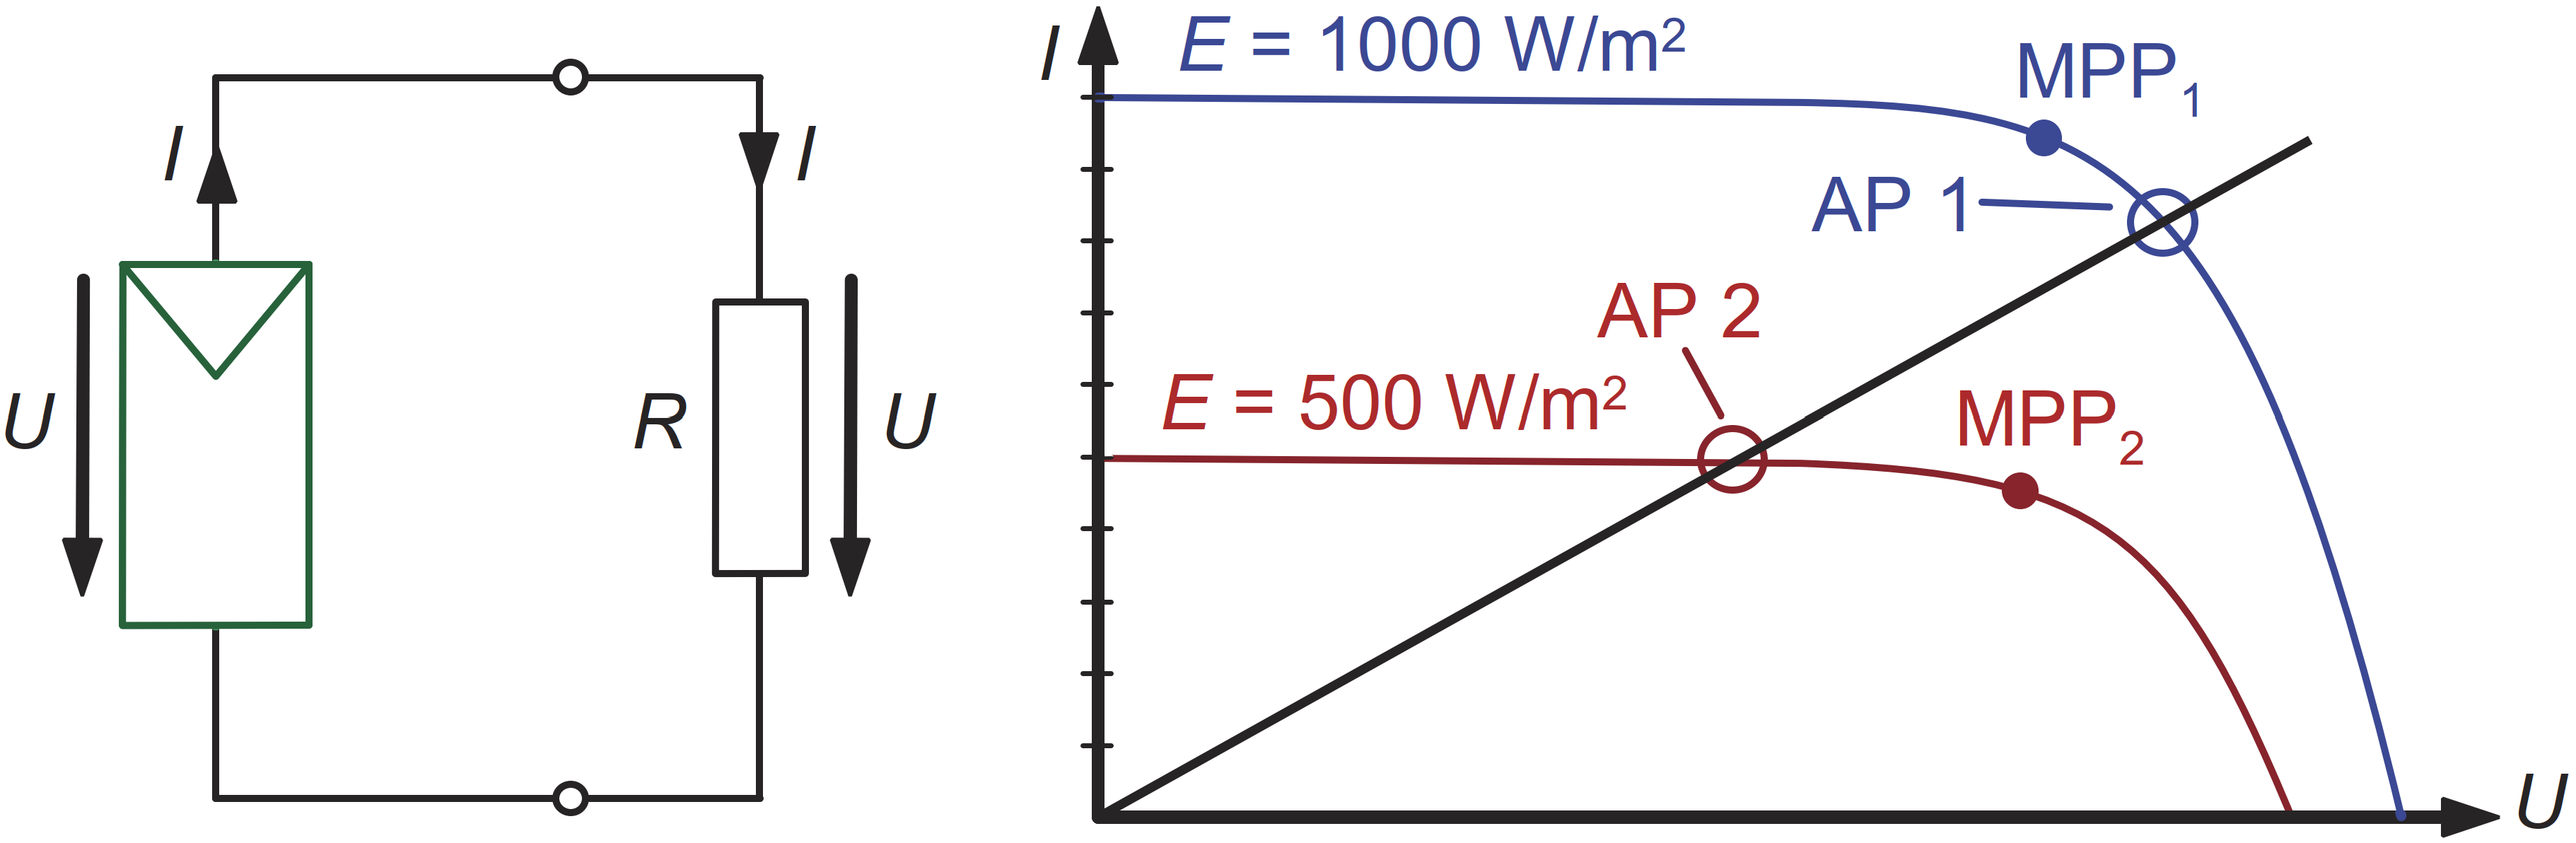
\includegraphics[width=0.95\columnwidth]{images/PV-Generator_unter_Last.png}



\subsection{Tiefstellsetzer, Buck-Converter}
\subsubsection{Einfaches Modell}
\begin{minipage}[t]{0.48\columnwidth}
    \myul{\textbf{Vereinfachtes Schema}}\\
\end{minipage}
\hfill
\begin{minipage}[t]{0.48\columnwidth}
    \myul{\textbf{Pulsweitenmodulation PWM}}\\
\end{minipage}

\begin{minipage}[c]{0.48\columnwidth}
    \begin{center}
        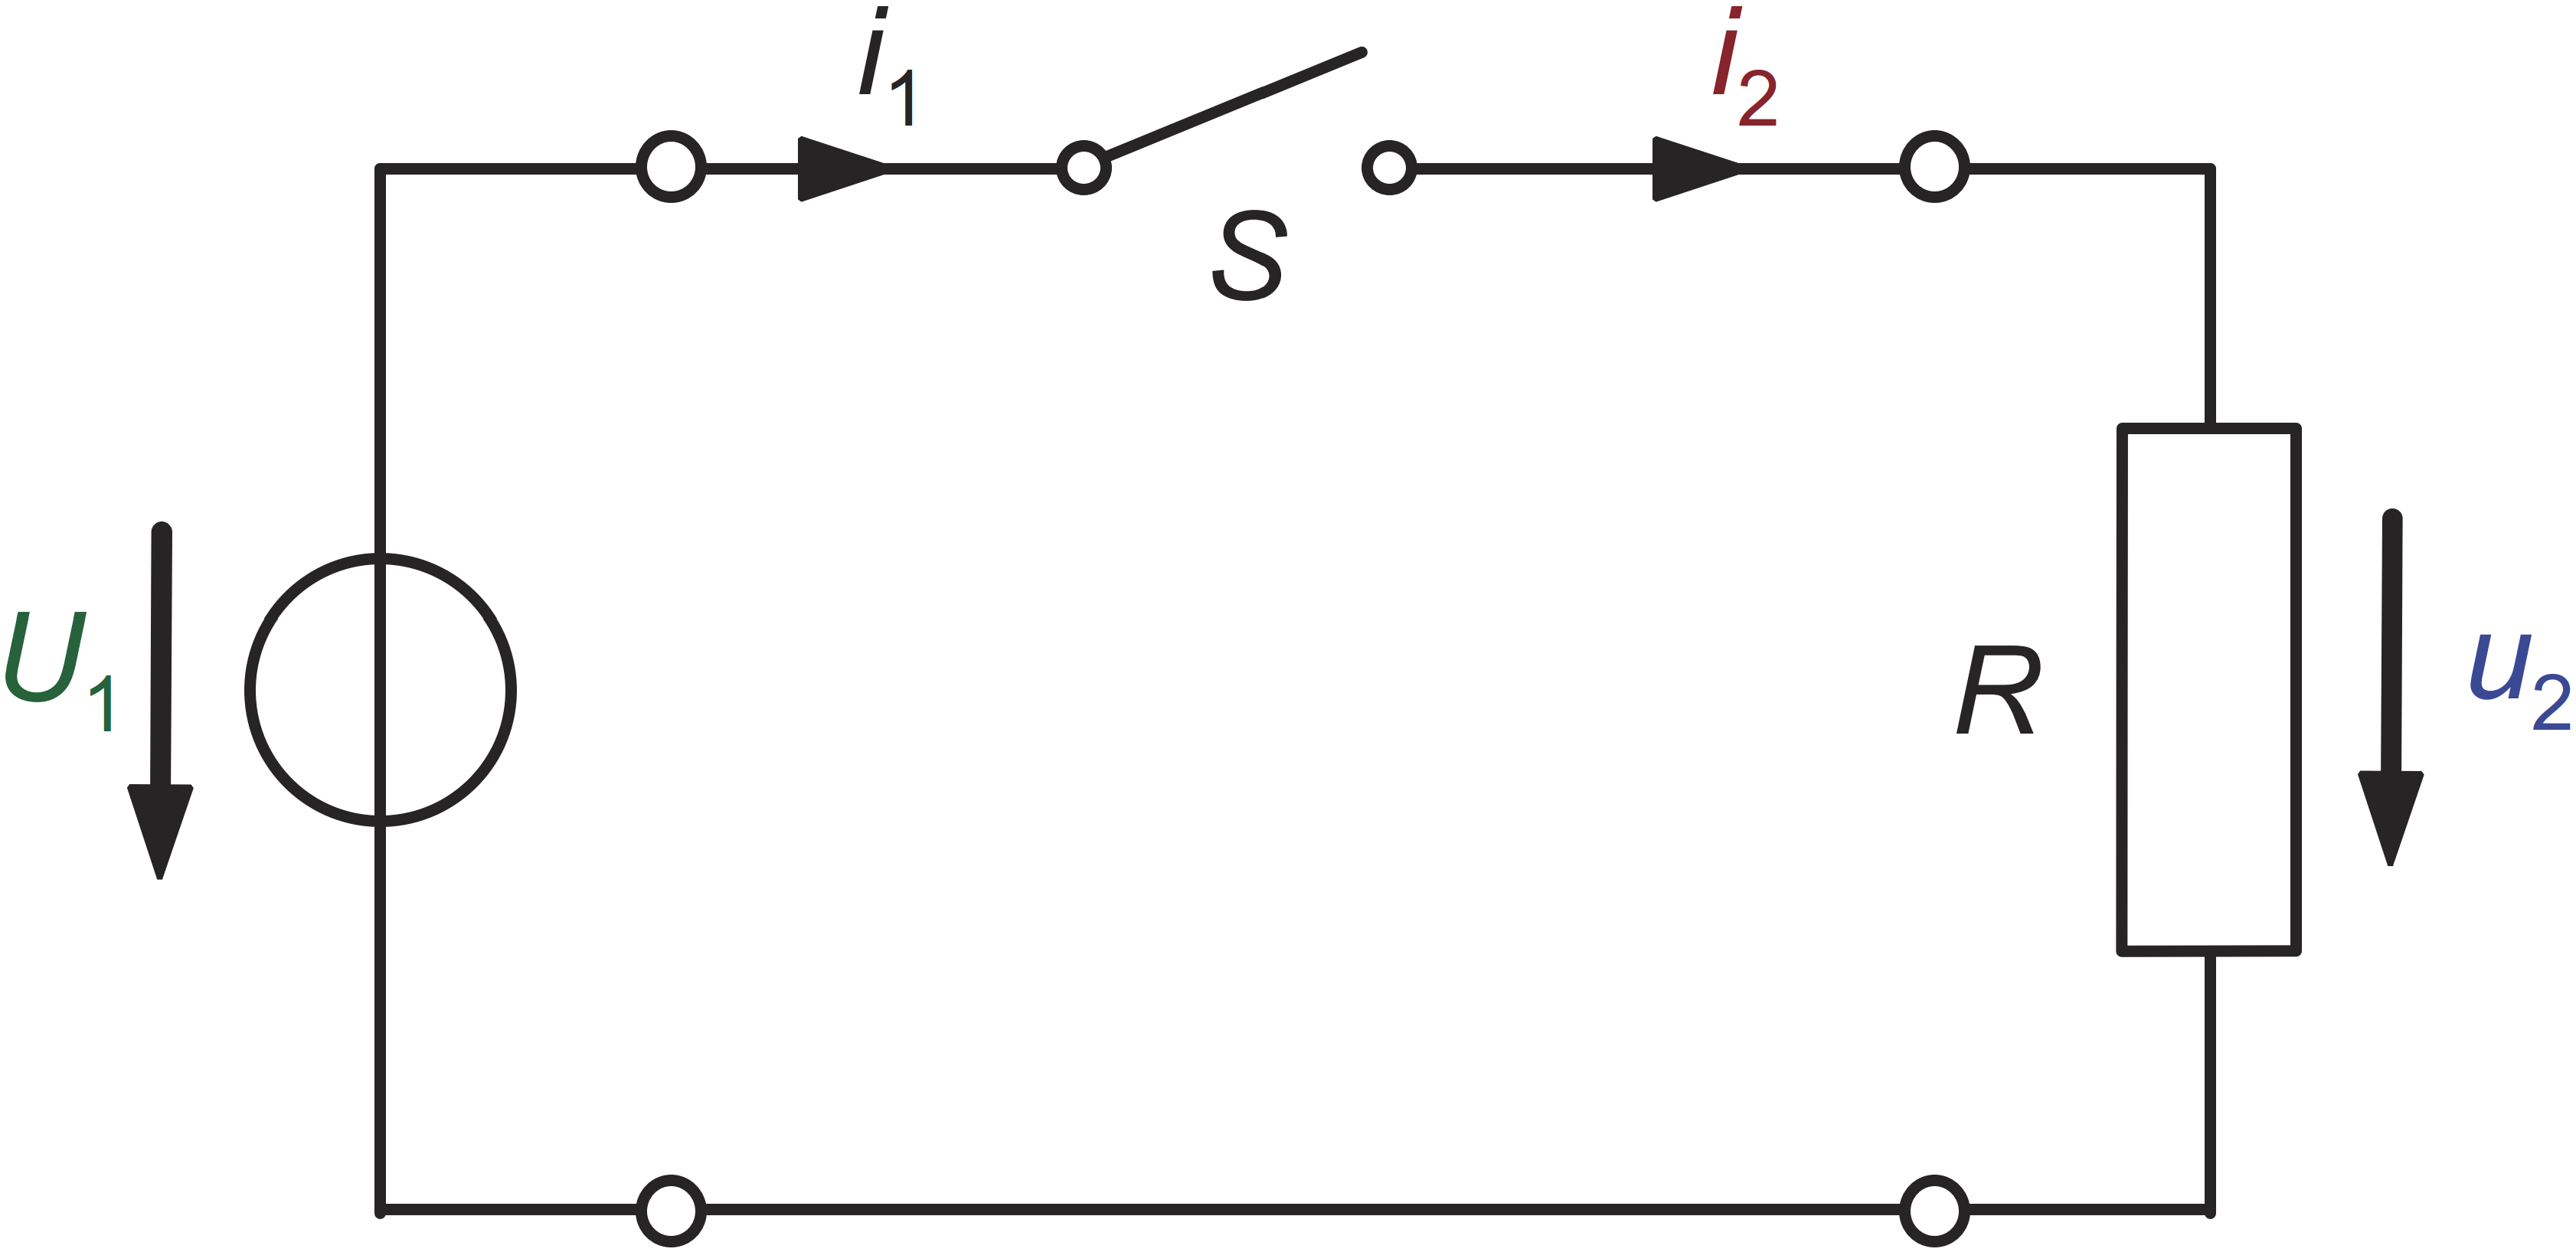
\includegraphics[width=1\columnwidth]{images/Tiefsetzsteller_Vereinfacht.png} 
    \end{center}
    
\end{minipage}
\hfill
\begin{minipage}[c]{0.48\columnwidth}
    \begin{center}
        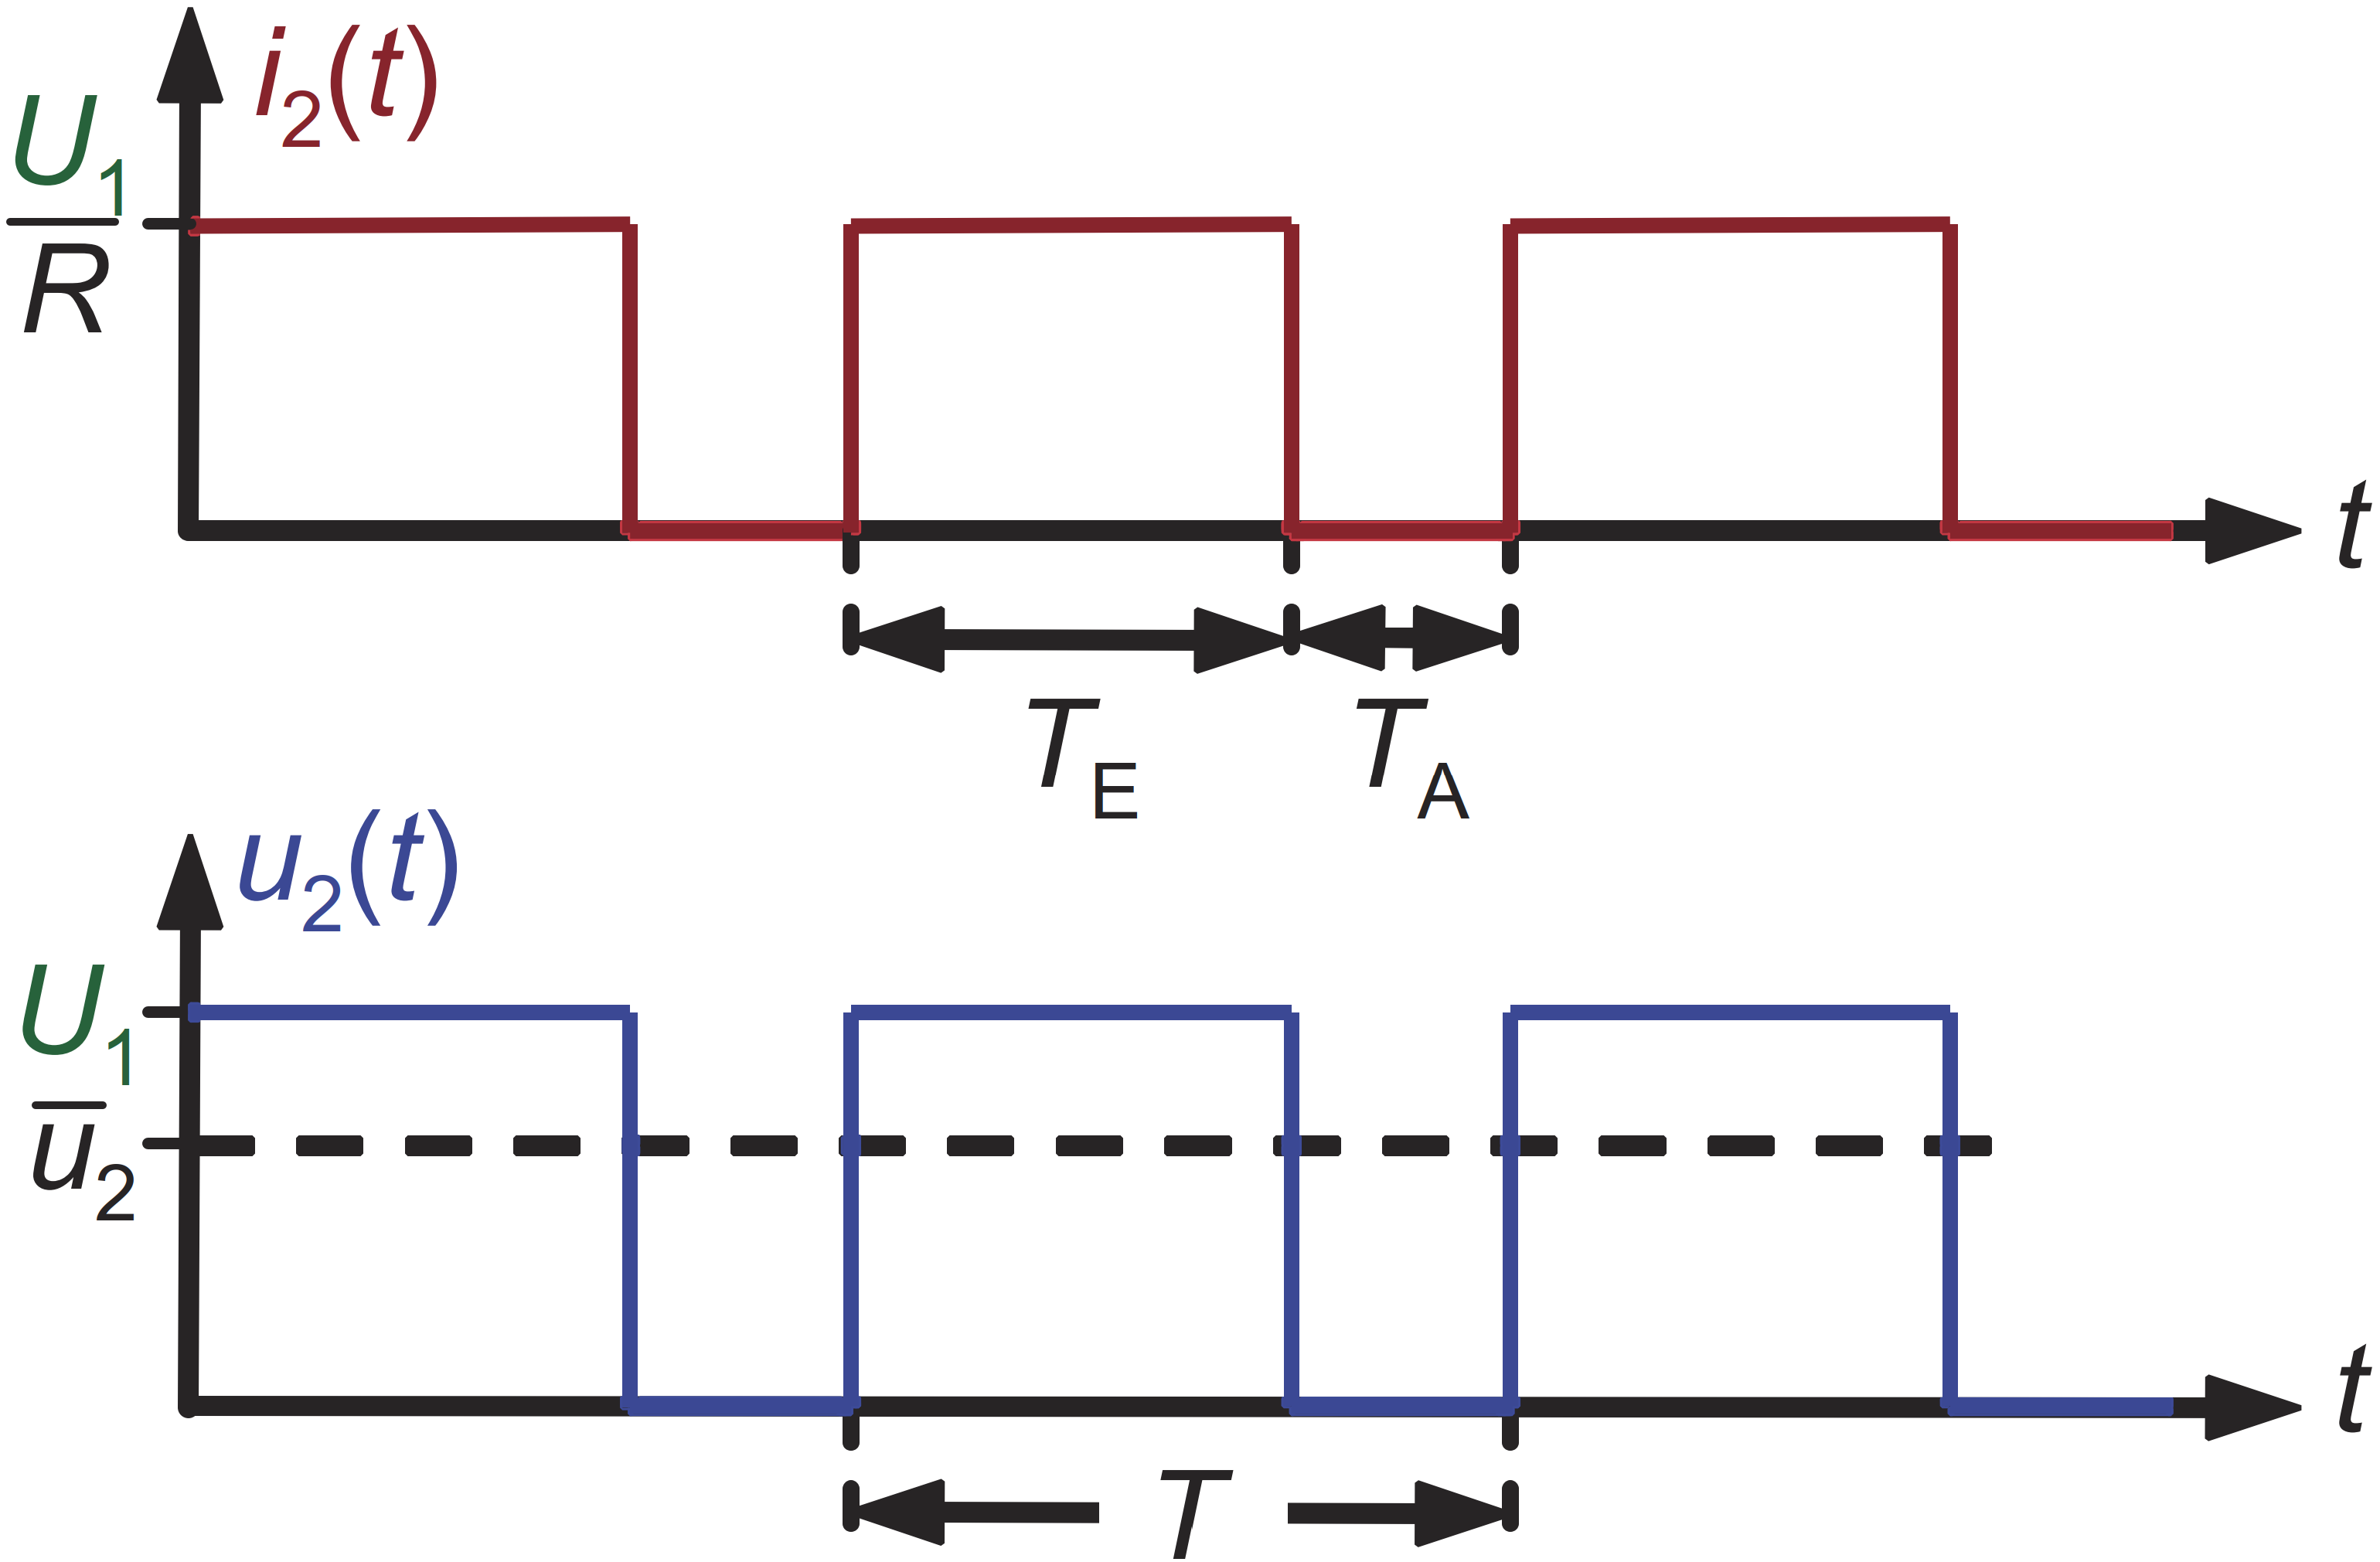
\includegraphics[width=0.95\columnwidth]{images/Tiefsetzsteller_DutyCycle.png}
    \end{center}
\end{minipage}



$
\boxed{
\bar{u}_2 = \frac{T_E}{T} \cdot U_1 = a \cdot U_1
}
$
\quad
$
\boxed{
a = \frac{T_E}{T}
}
$
\quad
$
\boxed{T = T_E +T_A}
$

\renewcommand{\arraystretch}{1.2}
\begin{tabular}{@{} l p{5cm} l @{}}
    $T$         & Periodendauer der PWM                     \dotfill & $s$ \\
    $T_E$       & Einschaltdauer der PWM                    \dotfill & $s$ \\
    $T_E$       & Ausschaltdauer der PWM                    \dotfill & $s$ \\
    $a$         & Tastgrad, Tastverhältnis, Duty Cycle      \dotfill & $-$ \\
    $U_1$       & Eingangsspannung                          \dotfill & $V$ \\
    $\bar{u}_2$ & Mittlere Ausgangsspannung                 \dotfill & $V$ \\
\end{tabular}


\subsubsection{Effektives Schema Tiefstellsetzer, Buck-Converter}
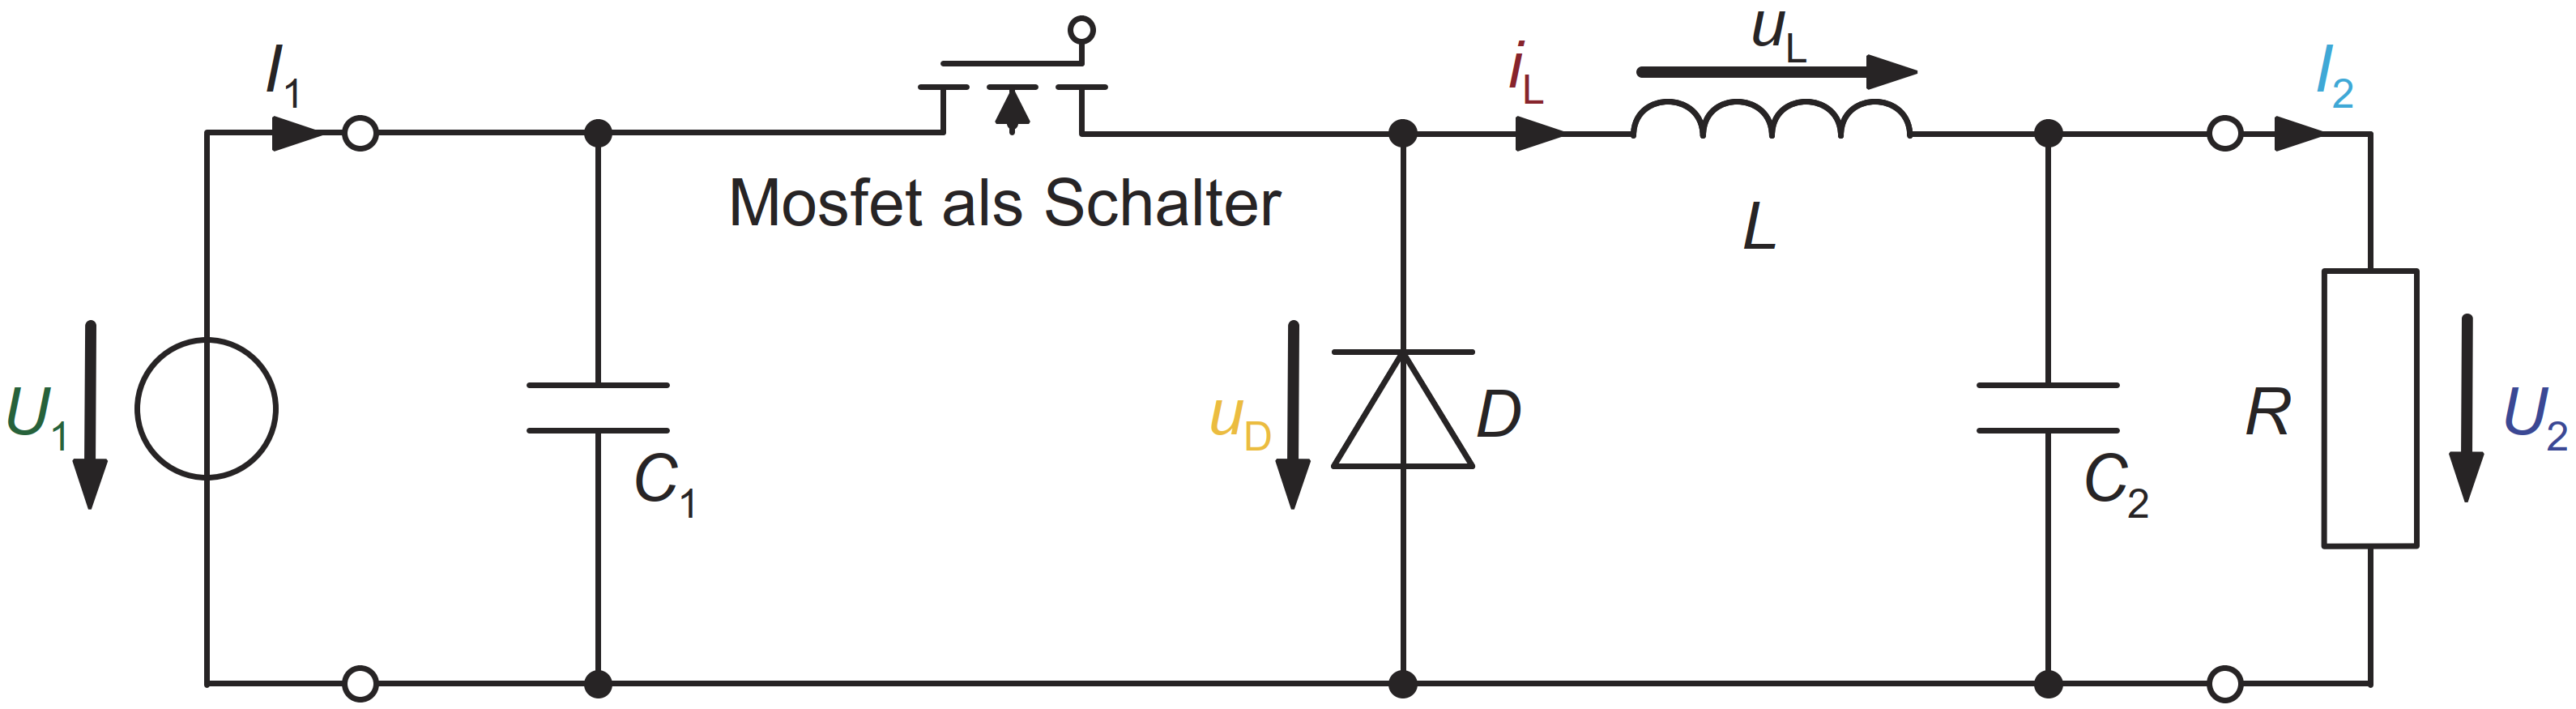
\includegraphics[width=1\columnwidth]{images/Tiefsetzsteller_1.png}

\vspace{0.25cm}

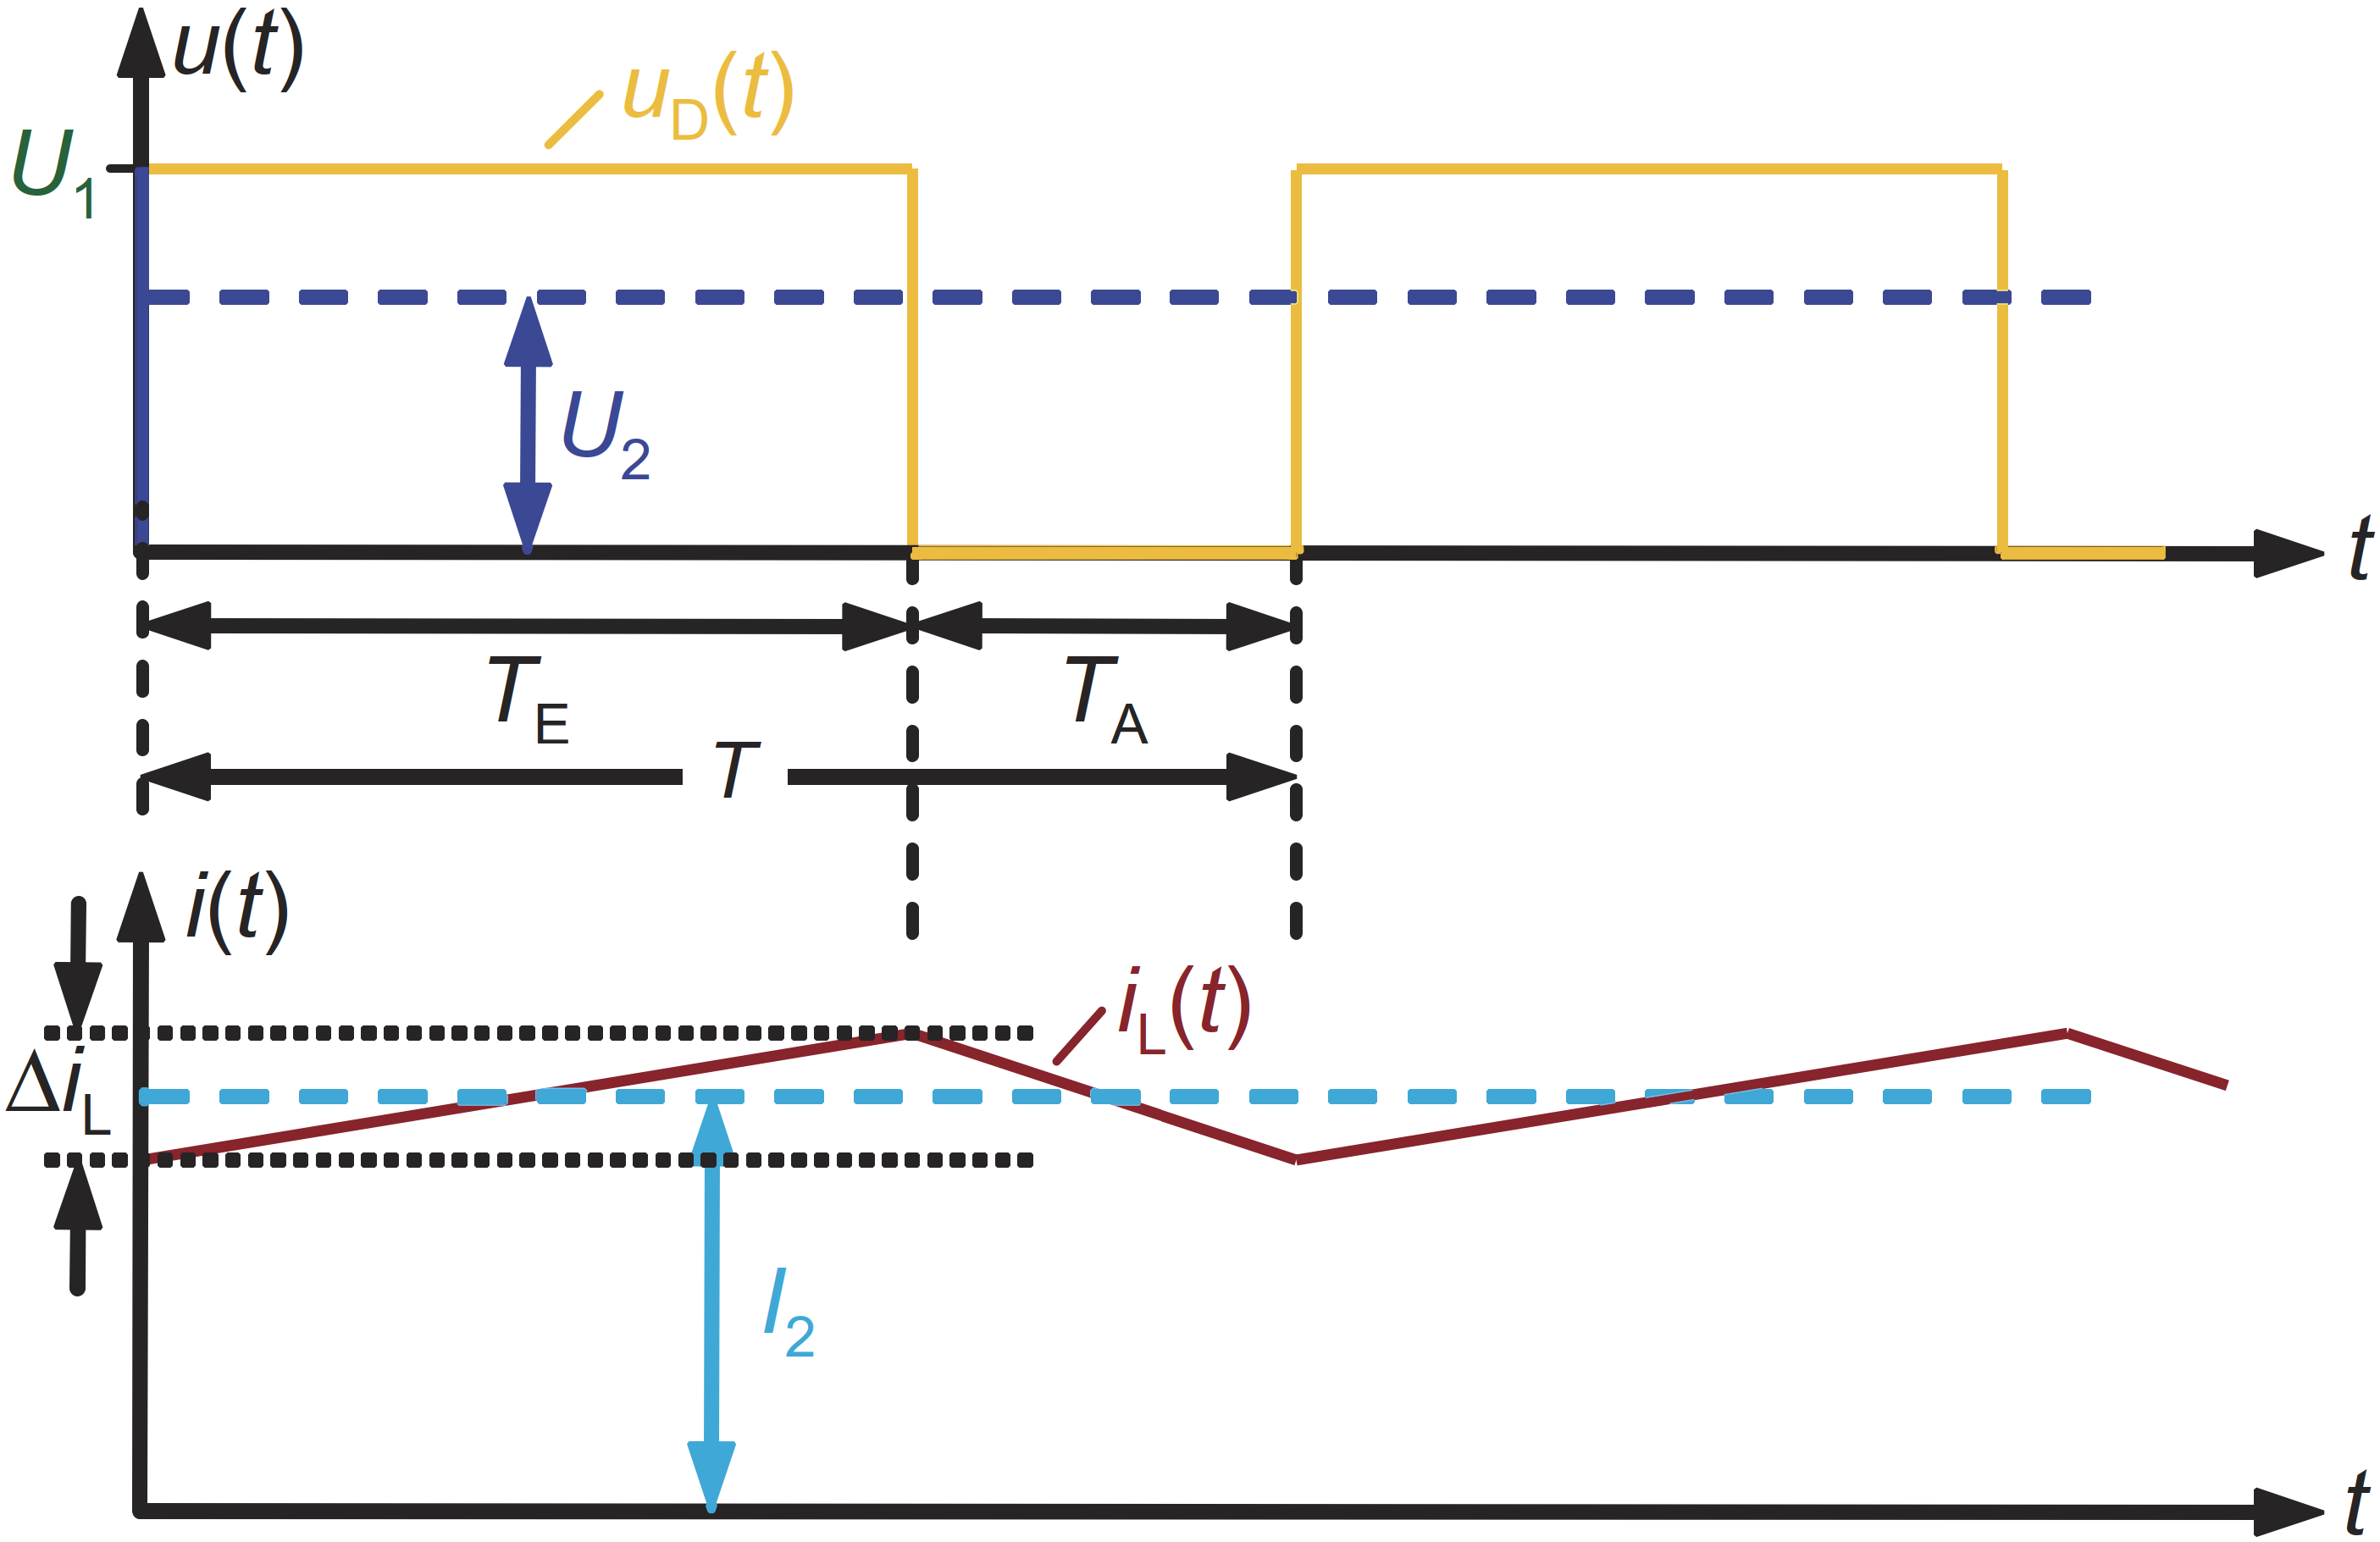
\includegraphics[width=0.8\columnwidth]{images/Tiefsetzsteller_2.png}

\vspace{0.25cm}

$
\boxed{u_D = U_1}
$
\quad
$
\boxed{u_L = u_D - U_2 = U_1 - U_2}
$
\quad
$
\boxed{u_L(t) = L \cdot \frac{\mathrm{d}i_L}{\mathrm{d}t}}
$
\quad
$
\boxed{U_2 = a \cdot U_1}
$

\vspace{0.25cm}

\begin{minipage}[t]{0.48\columnwidth}
    \myul{\textbf{Strom Anstiegsgeschwindigkeit ($T_E$)}}\\
    $
        \boxed{\frac{\mathrm{d}i_L}{\mathrm{d}t} = \frac{u_L}{L} = \frac{U_1 - U_2}{L}}
    $
    \quad
    $t \in [0, T_E]$
\end{minipage}
\hfill
\begin{minipage}[t]{0.48\columnwidth}
    \myul{\textbf{Strom Abfallstiegsgeschwindigkeit ($T_A$)}}\\
    $
        \boxed{\frac{\mathrm{d}i_L}{\mathrm{d}t} = \frac{u_L}{L} = \frac{-U_2}{L}}
    $
    \quad
    $t \in [T_E, T_A]$
\end{minipage}

\vspace{0.25cm}

\renewcommand{\arraystretch}{1.2} % Erhöht Zeilenhöhe für bessere Lesbarkeit
\begin{tabular}{@{} l p {6cm} l @{}}
    $[u_D]$   & Spannung an der Diode                      \dotfill & $V$ \\
    $[U_1]$   & Eingangsspannung                           \dotfill & $V$ \\
    $[U_2]$   & Ausgangsspannung                           \dotfill & $V$ \\
    $[u_L]$   & Spannung an der Spule (Drossel)            \dotfill & $V$ \\
    $[i_L]$   & Strom durch die Spule                      \dotfill & $A$ \\
    $[L]$     & Induktivität der Spule                     \dotfill & $H$ \\
    $[T_E]$   & Einschaltdauer                             \dotfill & $s$ \\
    $[a]$     & Tastgrad                                   \dotfill & $-$ \\
\end{tabular}





\subsection{Hochstellsetzer, Boost-Converter}

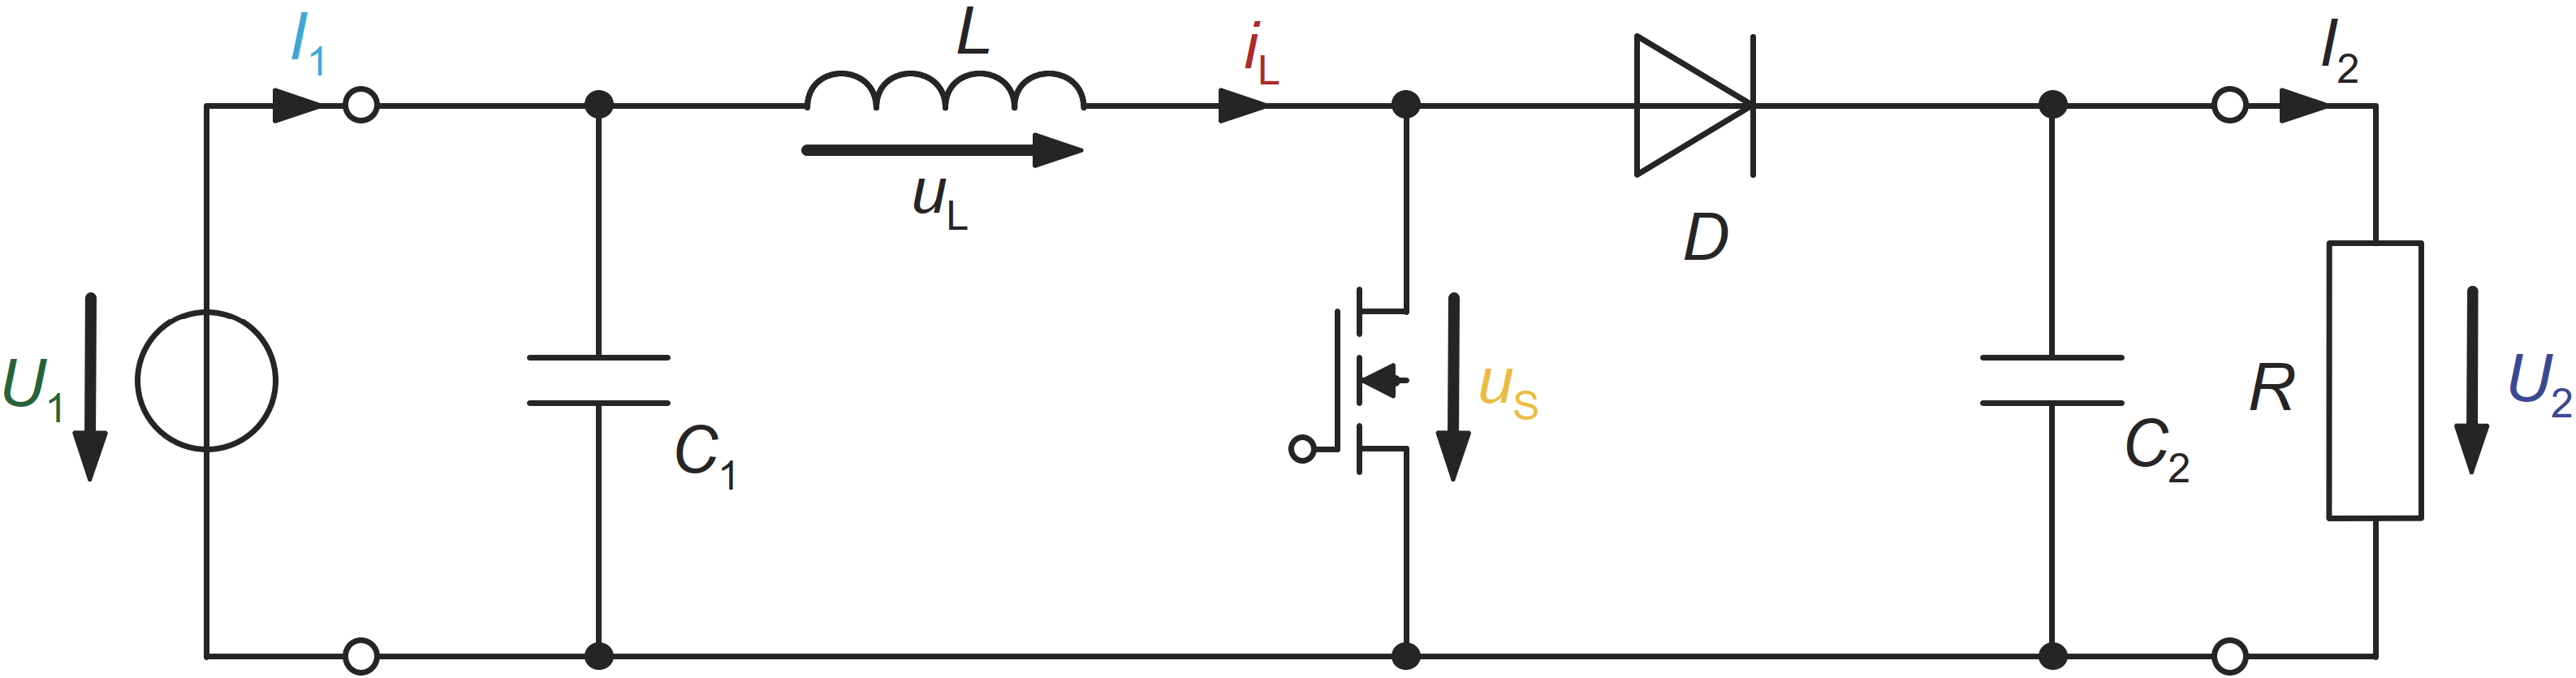
\includegraphics[width=1\columnwidth]{images/Hochstellsetzer_1.png}

\vspace{0.25cm}

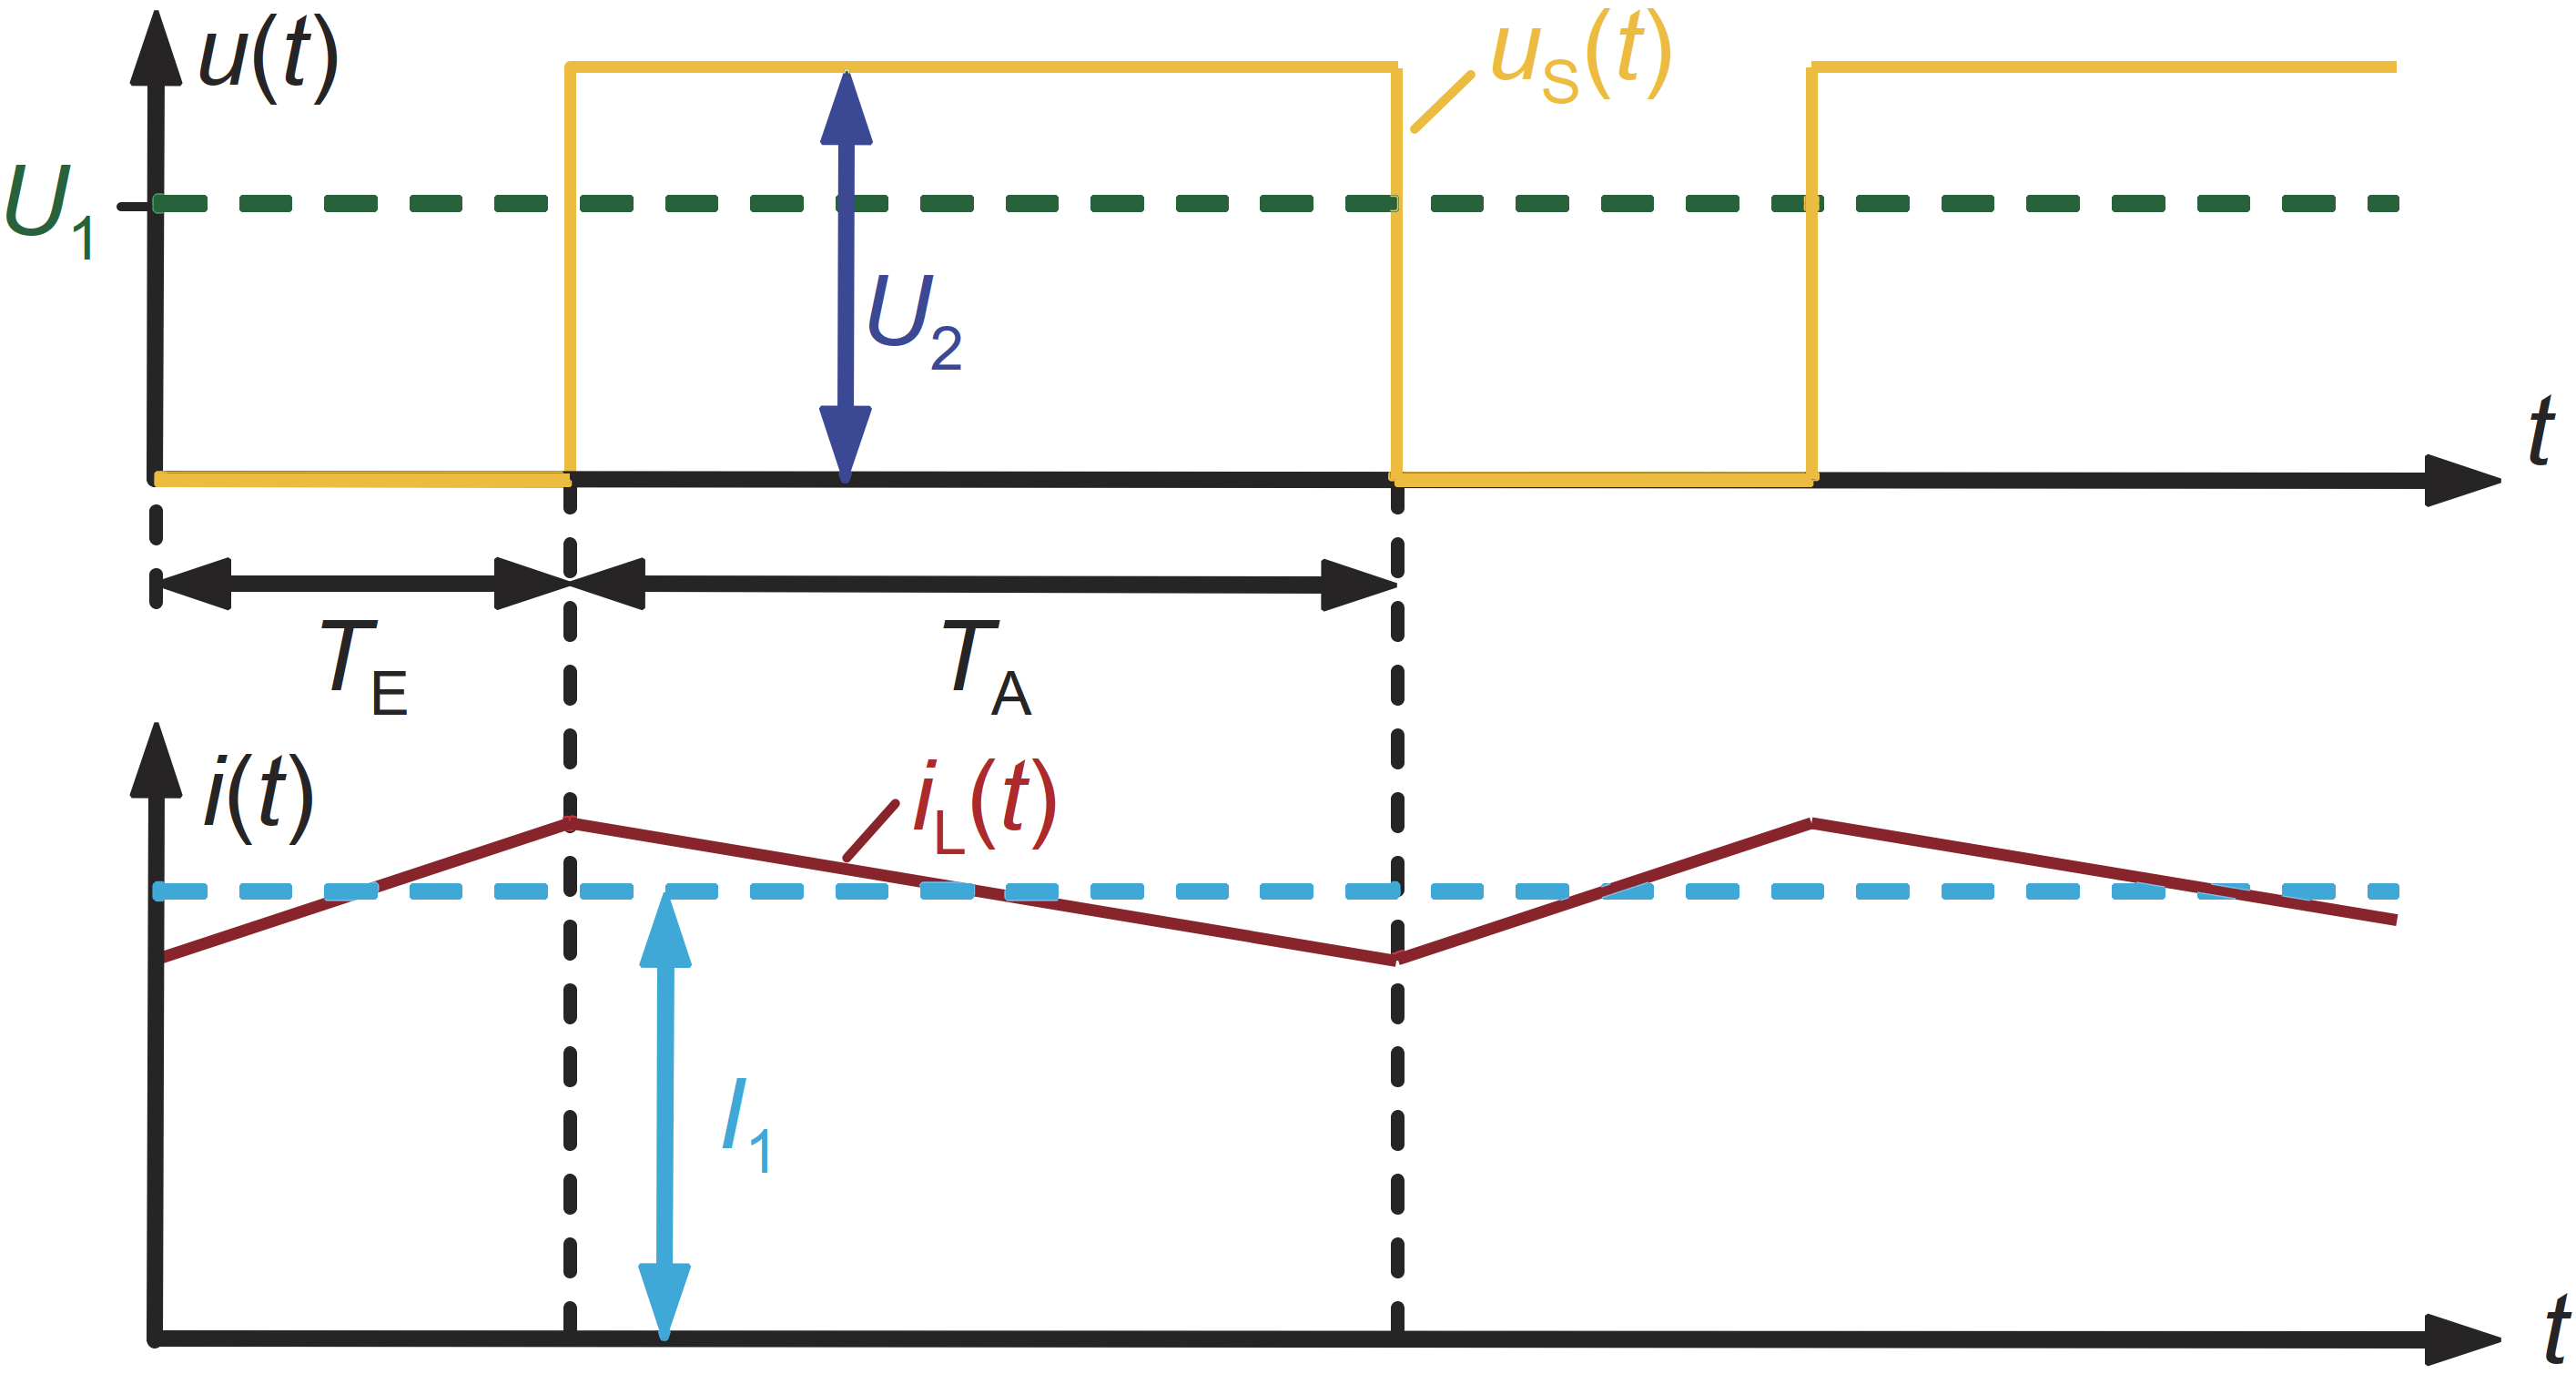
\includegraphics[width=0.8\columnwidth]{images/Hochstellsetzer_2.png}

\vspace{0.25cm}


Nach der Zeitdauer $T_E$ wird der Transistor gesperrt. Die Drossel versucht, ihren Strom aufrecht zu erhalten. Wir nehmen an, dass $U_2 > U_1$ ist. In diesem Fall treibt die Drossel den Strom langsam absinkend über die Diode $D$ auf den Ausgang.

Die Spannung an der Drossel ergibt sich zu:



\textbf{\myul{Während $T_E$}}

$
\boxed{\frac{\mathrm{d}i_L}{\mathrm{d}t} = \frac{u_L}{L} = \frac{U_1}{L}}
$

\textbf{\myul{Während $T_A$}}

$
\boxed{u_L = U_1 - U_2}
$
\quad
$
\boxed{\frac{\mathrm{d}i_L}{\mathrm{d}t} = \frac{u_L}{L} = \frac{U_1 - U_2}{L}}
$
\quad
$
\boxed{U_2 = U_1 - u_L}
$




\vspace{1em}
\renewcommand{\arraystretch}{1.2} % Erhöht Zeilenhöhe für bessere Lesbarkeit
\begin{tabular}{@{} l p {6cm} l @{}}
    $[U_1]$   & Eingangsspannung                           \dotfill & $V$ \\
    $[U_2]$   & Ausgangsspannung                           \dotfill & $V$ \\
    $[u_L]$   & Spannung an der Drossel                    \dotfill & $V$ \\
    $[i_L]$   & Strom durch die Spule                      \dotfill & $A$ \\
    $[L]$     & Induktivität                               \dotfill & $H$ \\
    $[T_E]$   & Einschaltdauer                             \dotfill & $s$ \\
\end{tabular}



\subsection{Berechnung der Ausgangsspannung}

Aus der Beziehung zwischen Ein- und Ausgangsspannung ergibt sich zunächst:

\[
\boxed{U_2 \cdot T_A = U_1 \cdot T}
\]

Daraus folgt für die Ausgangsspannung:

\[
\boxed{U_2 = \frac{T}{T_A} \cdot U_1 = \frac{T}{T - T_E} \cdot U_1 = \frac{1}{1 - \frac{T_E}{T}} \cdot U_1 = \frac{1}{1 - a} \cdot U_1}
\]

\vspace{1em}
\renewcommand{\arraystretch}{1.2} % Erhöht Zeilenhöhe für bessere Lesbarkeit
\begin{tabular}{@{} l p {6cm} l @{}}
    $[U_1]$   & Eingangsspannung                       \dotfill & $V$ \\
    $[U_2]$   & Ausgangsspannung                       \dotfill & $V$ \\
    $[T]$     & Periodendauer                          \dotfill & $s$ \\
    $[T_E]$   & Einschaltdauer                         \dotfill & $s$ \\
    $[T_A]$   & Ausschaltdauer ($T_A = T - T_E$)       \dotfill & $s$ \\
    $[a]$     & Tastgrad ($a = \frac{T_E}{T}$)         \dotfill & $-$ \\
\end{tabular}

